\chapter{Architektur}
\label{cha:architektur}
In diesem Kapitel werden architektonische Entscheidungen, anhand der Anforderung, den Umsetzungsmöglichkeiten und Vor- sowie Nachteilen, erläutert. Gleichzeitig werden weitere, detailliertere Anforderungen erstellt, die aus Entscheidungen resultieren. Zu Beginn werden grundlegende Entscheidungen beschrieben und im weiteren Verlauf der Arbeit detailliertere Einsichten in die Software gegeben.
\section{Grundsätzliche Entscheidungen}
\label{sec:grund_entscheidungen}
Wie aus der Anforderung [QUELLE] hervorgeht muss ein Produkt elektronisch erfasst werden. 
\\
Grundsätzlich gibt es verschiedene Möglichkeiten ein Produkt zu erfassen. 
Der Anwender könnte einen bestimmten Code für das jeweilige Produkt in die Brille eingeben, ob per Sprache oder per Hand sei zu diesem Zeitpunkt offen. Dies hätte allerdings den Nachteil, dass der Anwender für jedes Produkt einen Code merken müsste, dass gegen eine Entlastung des Mitarbeiters spricht.
\\
Eine andere Möglichkeit ist es den entsprechenden Artikel einzuscannen. Ein Barcode oder anderer Typ von Code ist im Normalfall immer gegeben, sodass an dieser Stelle kein Aufwand betrieben werden muss. Da die Brille eine integrierte Kamera besitzt, kann das Scannen des Artikels mithilfe der Brille direkt erfolgen. Der Vorteil daran ist, dass der Nutzer weiterhin ohne seine Hände aktiv zu nutzen arbeitet und keine weiteren Gerätschaften mittragen muss. Wie praktisch das Einscannen mithilfe der Brille ist und wie gut die Brillenkamera geeignet ist, soll in dieser Arbeit außer Acht gelassen werden, und das grundlegende Prinzip genutzt bzw. erforscht werden. 
Allerdings soll die Software so aufgebaut werden, dass ein umschalten zu externen Scannern möglich ist, damit die Praktikabilität erprobt werden kann.
\\
Laut Anforderung [Quelle] soll eine Zuordnung zwischen Code und Produkt erreicht werden.
Auch an dieser Stelle gibt es verschiedene Möglichkeiten. 
Dieses Mapping kann entweder auf der Brille erfolgen oder auf einer externen Komponente. Der Nachteil daran das Mapping auf der Brille durchzuführen ist, dass alle Daten dann auf der Brille gespeichert sein müssten. Dies kostet schon bei entsprechend großer Anzahl von Produkten viel Speicherplatz, der nur begrenzt zur Verfügung steht. Außerdem muss die Brille dann die Zuordnung selbst durchführen, was entsprechend viel Rechenleistung kostet, welche auch nur begrenzt verfügbar ist. Sofern das Mapping auf der Smartglass geschieht und die Daten somit auf der Smartglass gespeichert werden und dann mehrere Smartglasses in Betrieb sind, muss bei eine Aktualisierung jede Brille einzeln aktualisiert werden. 
Das Auslagern des Speicherns und des Zuordnens auf einen Datenbankserver behebt diese Nachteile, erfordert allerdings erst einmal das Aufstellen eines solchen Servers sowie einer Datenbank zur Speicherung der Daten. Zusätzlich ist eine Verbindung zwischen der Smartglass und dem entsprechendem Server notwendig. 
\\
Aufgrund von einer vorhandenen WLAN Anbindung der Smartglass ist dies kein Hindernis. Der einzige Flaschenhals könnte in der Datenübertragung zwischen Server und Brille auftreten. Allerdings ist der Austausch der Daten sehr gering. Im Prinzip verschickt die Smartglass einen gescannten Code mit der Anweisung den entsprechenden Artikel rauszusuchen an den Server. Eine solche einfache Abfrage verarbeiten Server in ausreichend hoher Geschwindigkeit und verschickt ebenfalls nur eine sehr geringe Datenmenge. Aus diesen Gründen wurde sich bei der Umsetzung für einen externen Server entschieden.
\\
Daraus ergeben sich folgende neue Anforderungen: 
\begin{itemize}
	\item Anforderung S1: Es muss ein Server aufgestellt werden.
	\item Anforderung S30: Es muss eine Kommunikationsschnittstelle zwischen Smartglass und Server geben.
\end{itemize}

Auch die geforderte Karte muss einerseits gemanagt und andererseits gespeichert werden. 
Das Erstellen und Verwalten einer solchen Karte ist auf der Brille nicht effizient und effektiv umsetzbar. Dazu ist das Display zu klein und die Handhabung nicht komfortabel genug. Da sich bereits entschieden wurde, einen Server einzubinden, kann das Management der Karten ebenfalls darauf erfolgen. Dazu ist eine geeignete Webanwendung notwendig, die es ermöglicht Regale zu erstellen, diese Regale mit Produkten zu füllen und folglich eine ganze Karte zu kreieren. Siehe Anforderung A10, A20, A30.
\\
Die folgende Grafik zeigt die entsprechenden Komponenten und deren Nutzer.
\begin{figure}[H]
	\centering
	{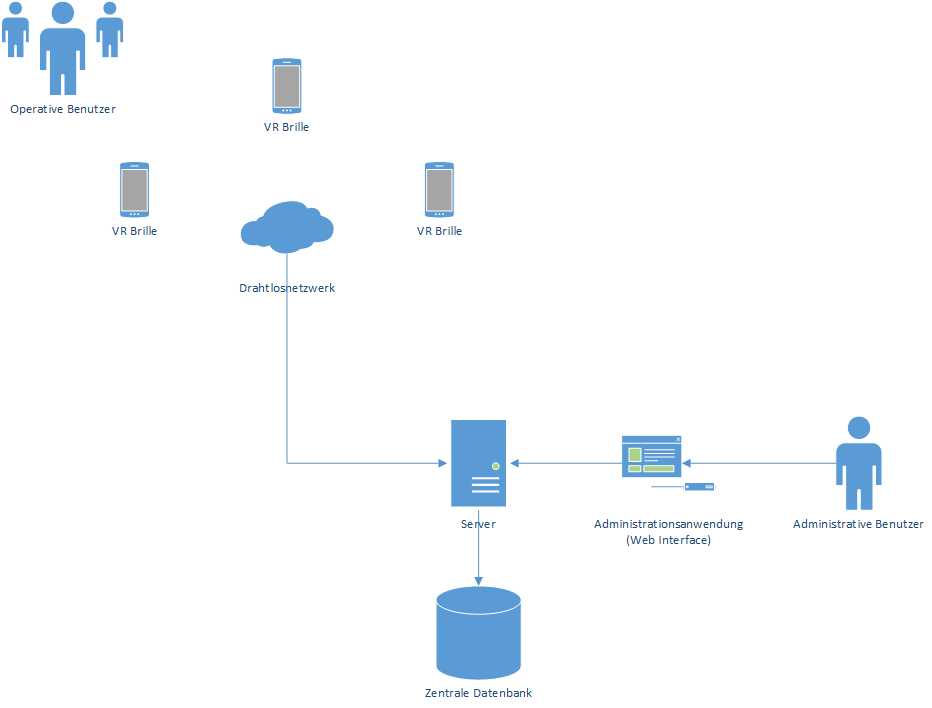
\includegraphics[scale=0.5]{Bilder/komponentendarstellung.png}}
	\caption{Netzwerkkomponentendiagramm}
	\label{fig:komponentendarstellung}
\end{figure}
Die Abbildung zeigt zusätzlich, dass verschiedene Smartglasses im Einsatz sind bzw. sein können. Dies macht auch Sinn, da bei entsprechend großer Filiale mehrere Mitarbeiter zum Beispiel Ware einräumen müssen. 
\\
Weiterhin stellt sich die Frage, wie die Smartglass mit der Karte in Kontakt tritt, damit daraus dem Mitarbeiter ein Bild angezeigt wird, wo die Ware eingeräumt werden soll. [Siehe Anforderung XY]
Dazu sind grundsätzlich zwei Varianten denkbar. Einerseits kann die Karte auf dem Server gelagert werden und die Brille agiert als Thin-Client. Dabei fragt die Smartglass beim Server mit dem Produktcode und der Anforderung nach Produktinformationen und gleichzeitig nach dem entsprechendem Bild, das angezeigt werden soll. 
\\
Der Vorteil an einer solchen Variante ist, dass die Brille dabei nicht belastet wird, was einerseits der Batterie zugutekommt und andererseits die Smartglass noch leichtgewichtiger wird. 
Der Nachteil einer solchen Variante zeigt sich bei dem Gedanken, dass das anzuzeigende Bild nicht nur das Regal selbst ist, sondern die Realität, also das aufgenommene Bild der integrierten Kamera. 
\\
Das bedeutet, dass die Kamera dauerhaft filmt. Dabei wird dem Nutzer nicht nur der Regalplatz selbst gezeigt, sondern auch der Weg dorthin beschrieben. Dies geschieht im optimalen Fall in Echtzeit.  
\\
Vor diesem Hintergrund bzw. diesem Ausblick, ist ein Austausch des Bildes mit dem Server nicht in entsprechend schneller Zeit möglich.
\\
Nachteil einer Umsetzung auf der Smartglass ist die Speicherung der Karte im Vorfeld. Da davon ausgegangen werden darf, dass sich nicht stündlich oder täglich die Positionen der Artikel oder gar die Regalaufstellung ändert, hält sich ein Aktualisierungsprozess in Grenzen und wird in Kauf genommen.
\\
Deshalb wurde sich dafür entschieden, dass die Karte mit allen Regalinformationen auf der Smartglass gespeichert wird. Die Smartglass erfragt beim Server nach dem einscannen des Code, das Produkt und dessen Regalplatz. Anschließend berechnet die Smartglass selbst den Regalplatz und erzeugt das Bild. 
\\
Zu Beginn soll die Abbildung bzw. das Miteinbeziehen der Realität außer Acht gelassen werden, und als Ausblick dienen. Allerdings soll die Software schon darauf ausgerichtet sein.
Aus dieser Entscheidung ergeben sich folgende, weitere Anforderungen: 
\begin{itemize}
	\item Anforderung B30: Es gibt eine Möglichkeit, die Karte auf der Brille zu speichern und zu aktualisieren. 
	\item Anforderung B40: Es gibt eine Möglichkeit, dass die Smartglass aus den Informationen der Karte und den Produktdaten das Bild des Regalplatzes berechnet.
	\item Anforderung B40.1: Es gibt eine Möglichkeit, dass das generierte Bild angezeigt wird.
\end{itemize}
Im Bezug auf die Warenannahme entstehen keine neuen grundsätzlichen Entscheidungen, da die bisher beschriebenen Anforderungen bzw. Entscheidungen auch die Anforderungen der Warenannahme realisieren können. 
Auch die Kundenzufriedenheit lässt sich anhand dessen realisieren. 
\\
Grundsätzlich lassen sich aus den bisherigen Anforderungen und den getroffenen Entscheidungen drei große Teilbereiche des Projekts identifizieren: 
\begin{enumerate}
	\item Smartglass
	\item Server
	\begin{itemize}
		\item Datenbank
		\item Kommunikationsmittel
	\end{itemize}
	\item Webanwendung
\end{enumerate}
Diese Teilbereiche sollen fortan im weiteren Verlauf der Arbeit einzeln weiter definiert und beschrieben werden.
\section{Section}
Kapitel \ref{cha:architektur}

\section{Another Section}
\subsection{bla}
\subsubsection{blabla}
\textbf{bla}\\
Hochkommata: \glqq asdas\grqq~~ sdasd\\

Neue Zeile: nur Backslash Backslash\\
sadas\\

Absatz\\

Aufzählung:
\begin{itemize}
	\item basd
	\item ...
\end{itemize}

\textit{\textbf{yxcyxcyxc}}
\underline{sdfsdf}
$\rightarrow$